\begin{frame}{Que voit-on sur un profil?}
    \centering
    \begin{figure}
        
\includegraphics[width=.4\textwidth]{Images/chloe_delaume.png}
        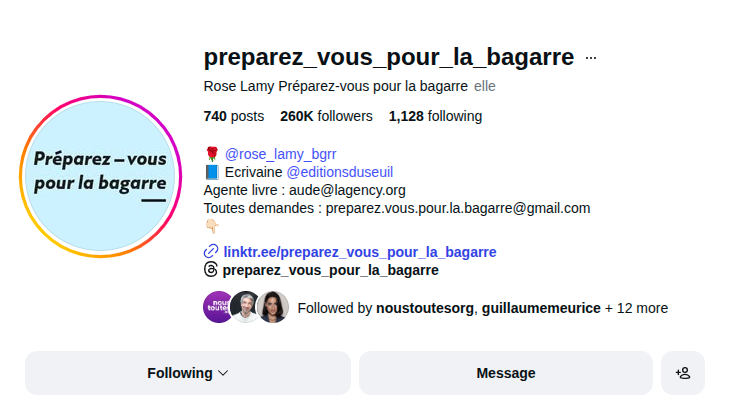
\includegraphics[width=.4\textwidth]{Images/preparez_vous_pour_la_bagarre.png}
    \end{figure}
\end{frame}
\begin{frame}{Les fonctions hétérogènes du profil}
    \begin{itemize}
        \item Utilisation en mode stratégie promotionnelle;
        \item Utilisation en mode création;
        \item Utilisation en mode réseau;
        \item Utilisation très perso
    \end{itemize}
    Les profils d'écrivains : très nombreux cas d'étude. Avec des degrés d'implication divers :

\end{frame}

\begin{frame}{Usage promotionnel}
    \centering
    \begin{figure}
        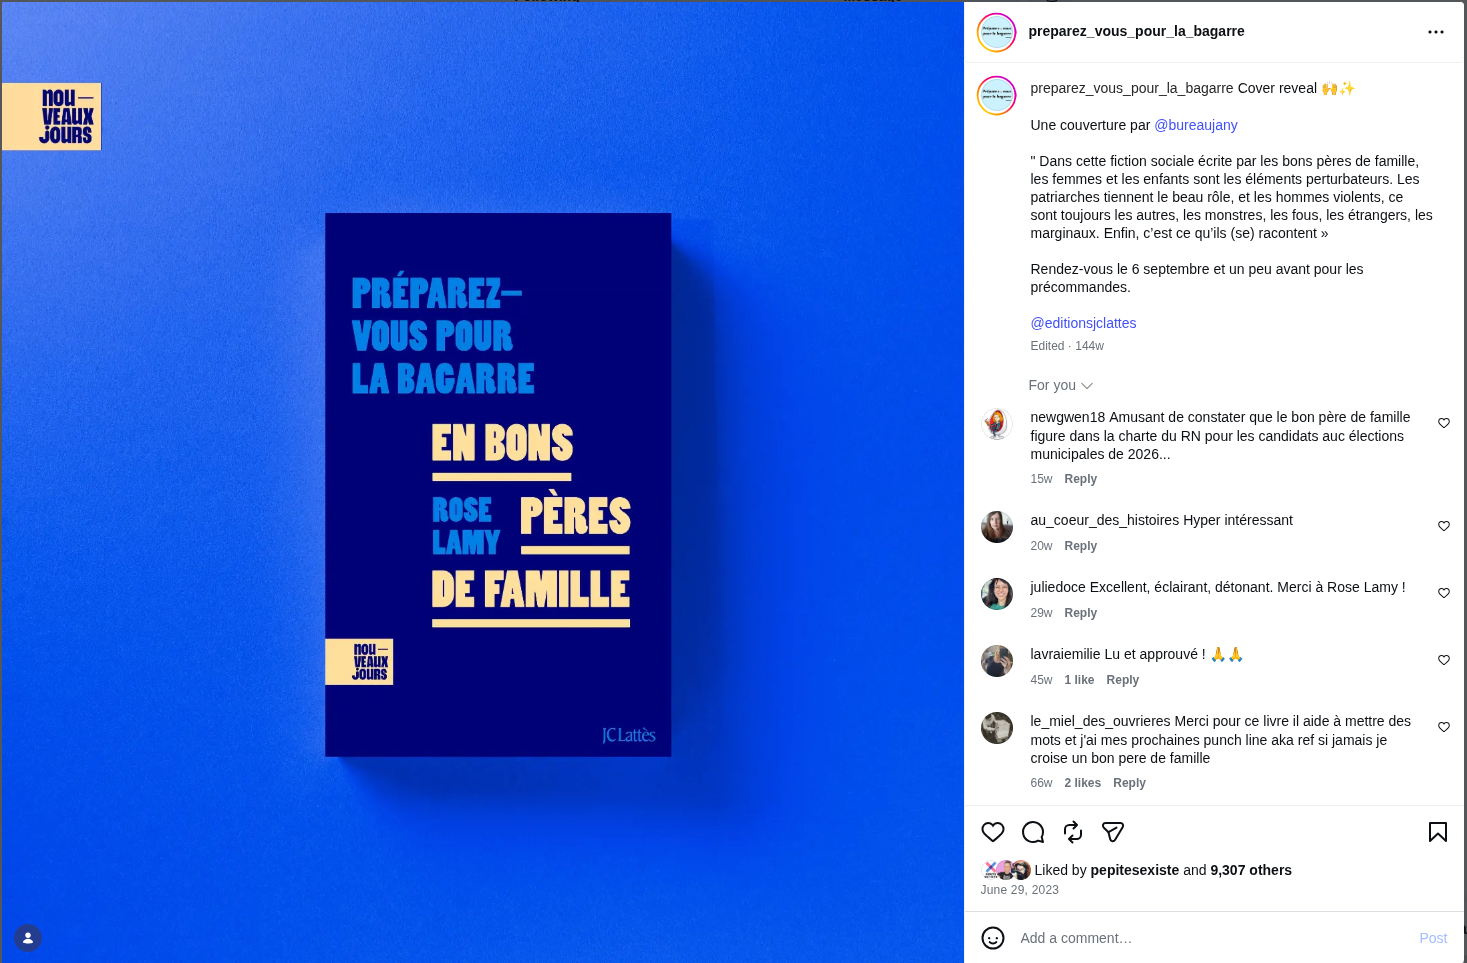
\includegraphics[width=.8\textwidth]{Images/promotion_insta.png}
    \end{figure}
\end{frame}

\begin{frame}{Usage créatif: récit de soi}
    \centering
    \begin{figure}
        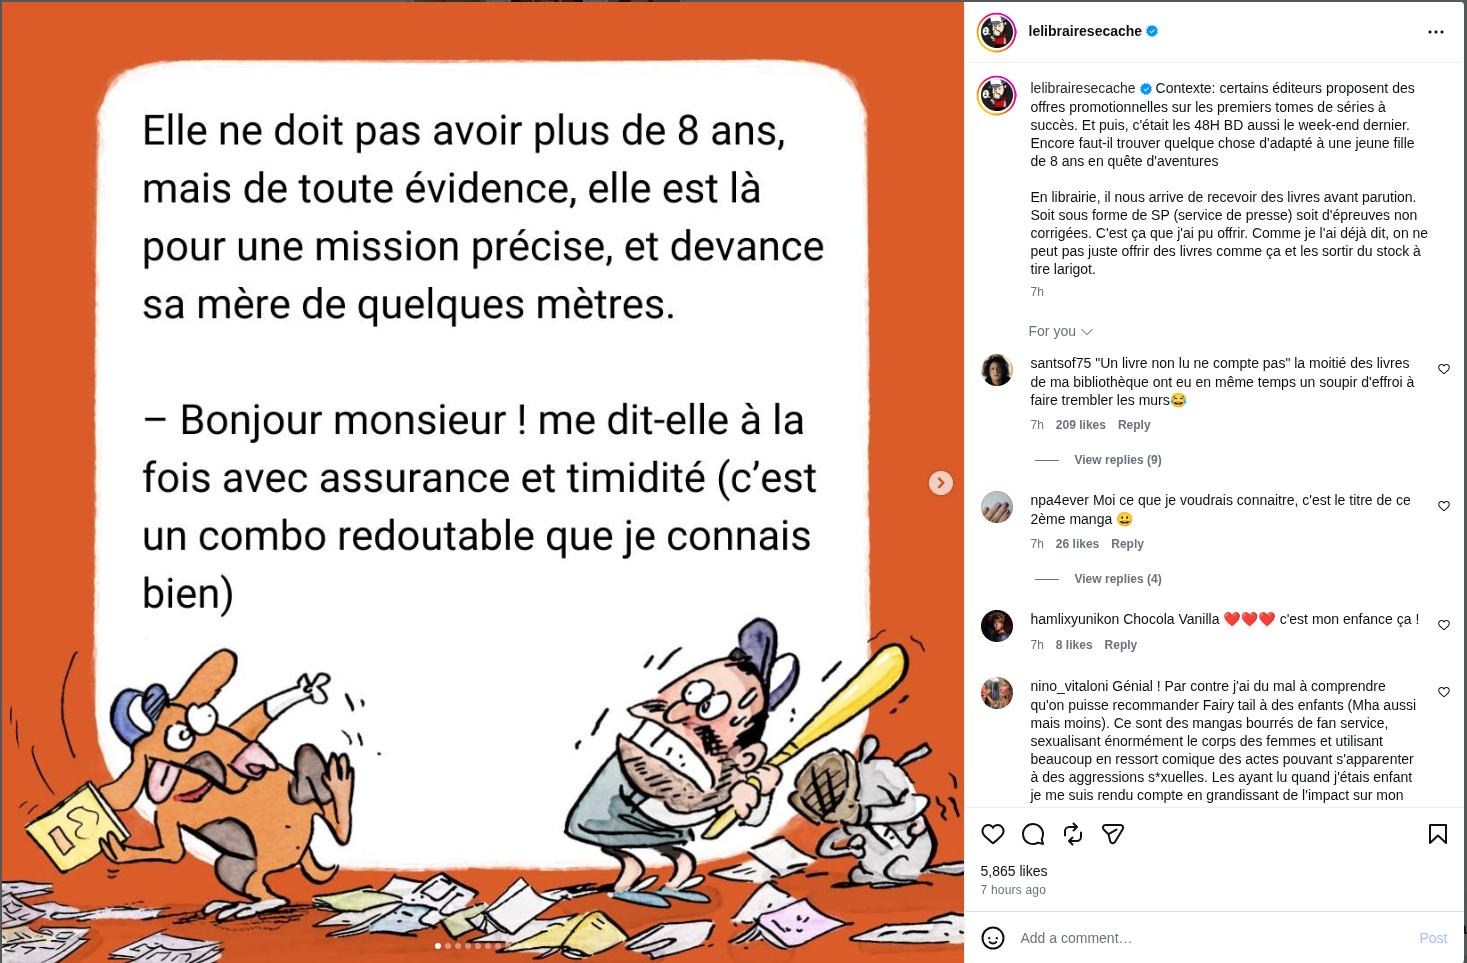
\includegraphics[width=.8\textwidth]{Images/libraire_se_cache.png}
    \end{figure}
\end{frame}

\begin{frame}{Usage créatif: le profil de fiction}
    \centering
    \begin{figure}
        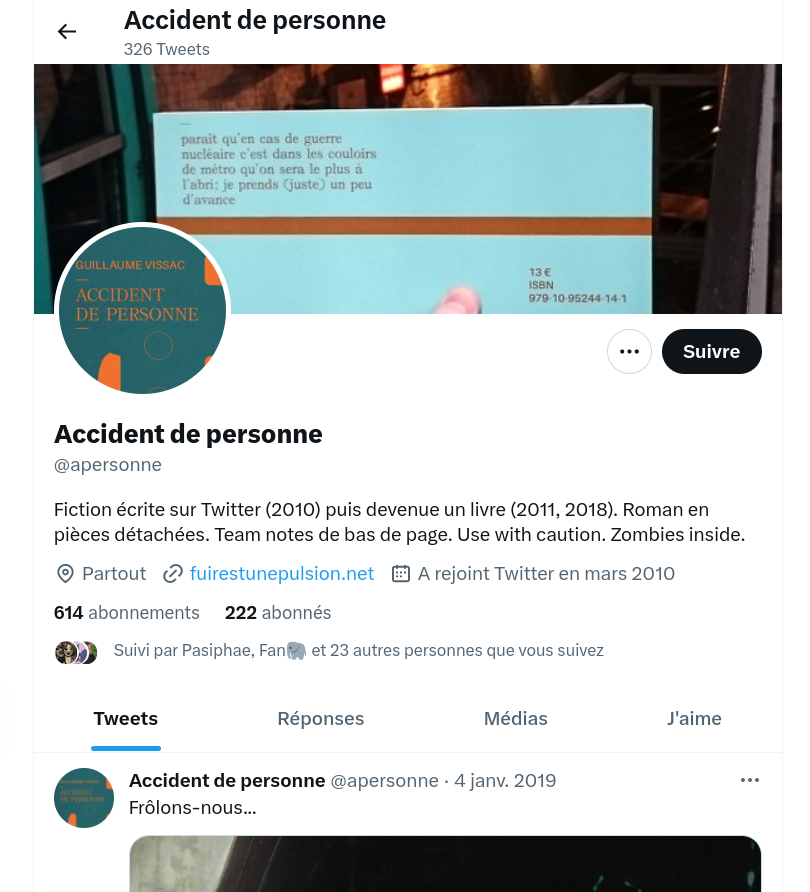
\includegraphics[width=.4\textwidth]{Images/AccidentPersonneVissac1.png}
        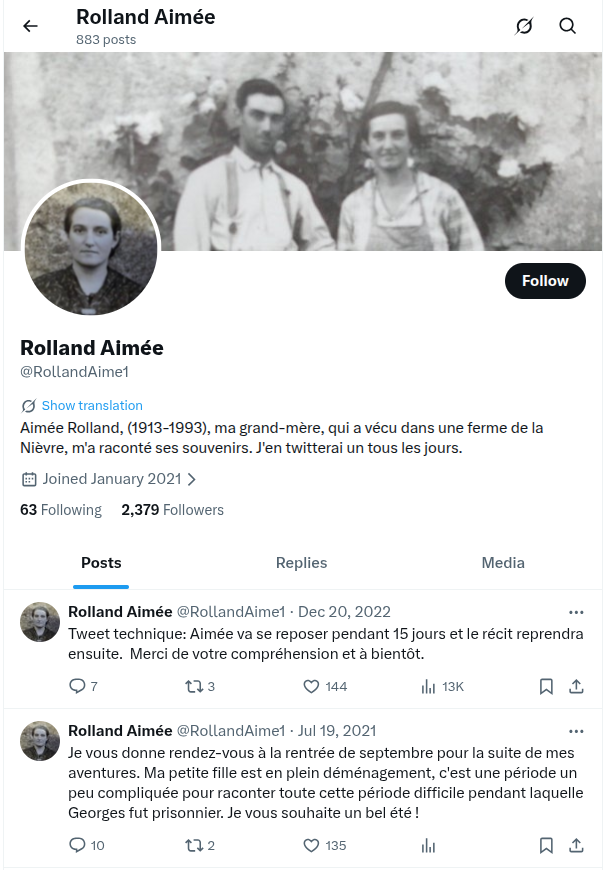
\includegraphics[width=.4\textwidth]{Images/aimée_rolland.png}
    \end{figure}
\end{frame}

\begin{frame}{Usage réseau}
    \centering
    \begin{figure}
        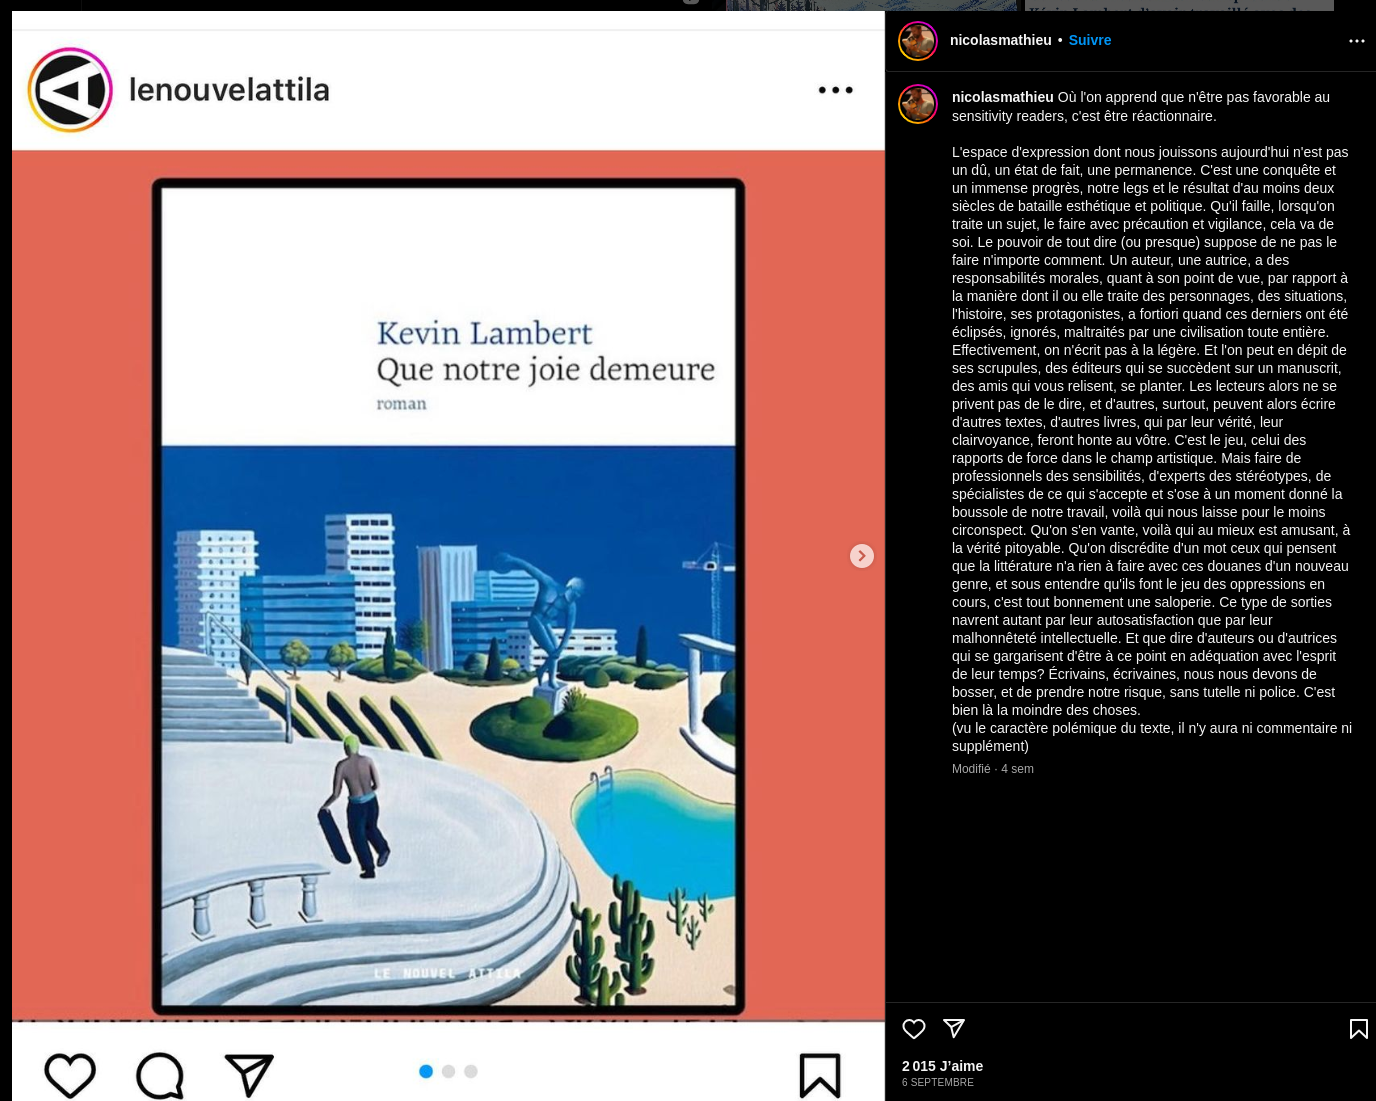
\includegraphics[width=.6\textwidth]{Images/NicolasMathieuPostInsta.png}
    \end{figure}
\end{frame}

\begin{frame}{Usage personnel}
    \centering
    \begin{figure}
        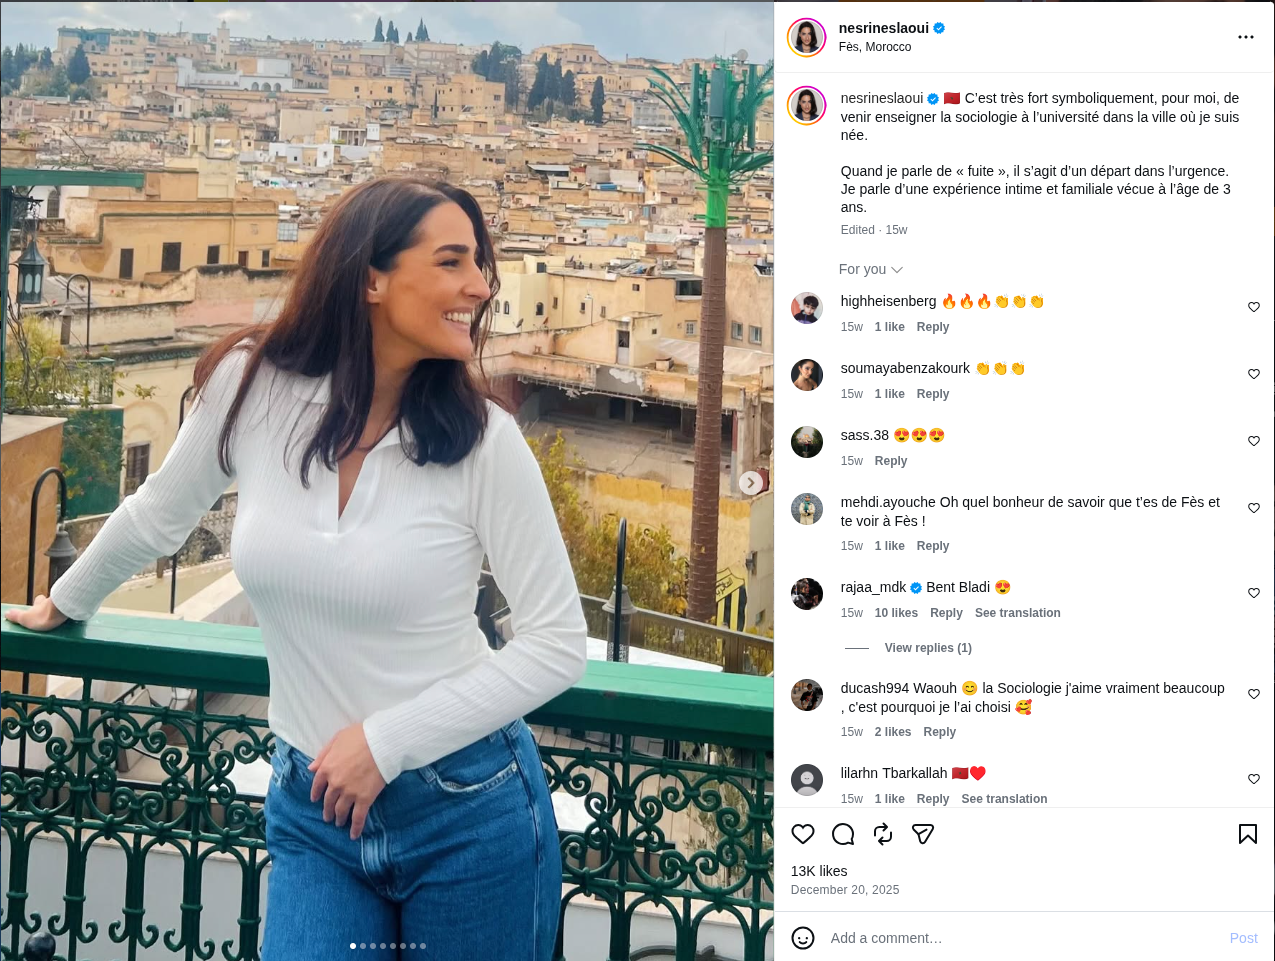
\includegraphics[width=.6\textwidth]{Images/nesrine_slaoui.png}
    \end{figure}
\end{frame}

\begin{frame}{Vers une transformation de la "présence sociale" de l'écrivain ?}
    \centering
    {\small \textit{«publier ne signifie plus du tout participer à la merveilleuse et abstraite sphère publique habermassienne. Bien au contraire, il s'agit bien souvent de multiplier son inscription dans des espaces publics. Une autre représentation se fait jour : celle d'une arène plus ou moins conflictuelle du littéraire où cette sphère publique entre en dialogue avec une multitude d'espaces publics où se déploient des littératures-brouhaha. La Littérature n'est plus alors qu'une des actualisations possibles du littéraire et de la publication. Encore une fois : pas de substitution, une addition.»}\\
\textbf{Ruffel Lionel, Brouhaha. Les mondes du contemporain}}
\end{frame}

\begin{frame}{De Twitter à X : les réseaux sociaux désertés ?}
    \centering
    \begin{figure}
        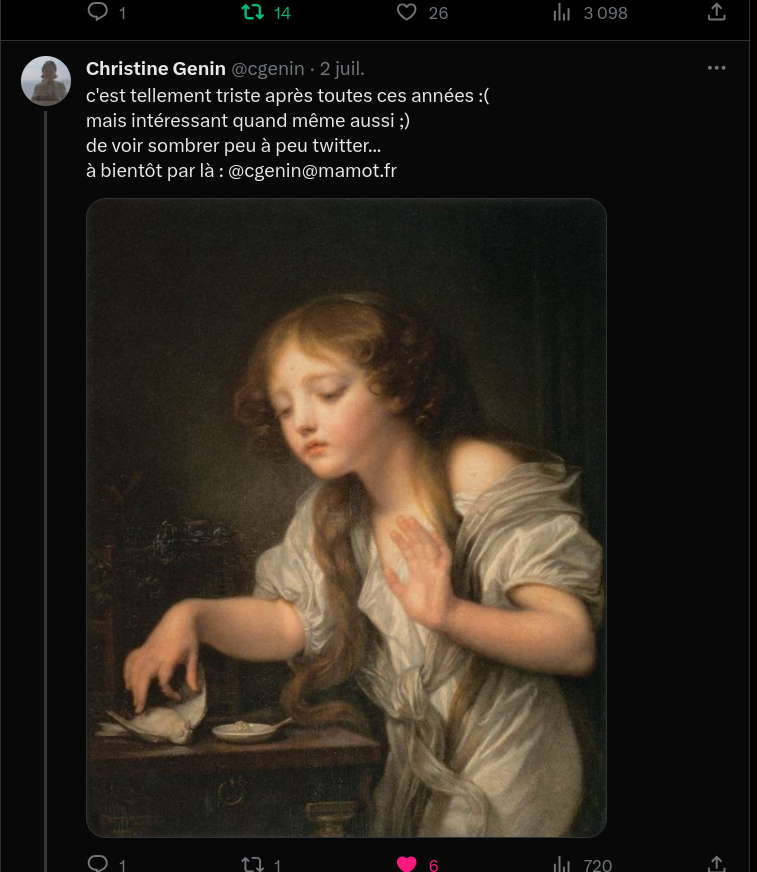
\includegraphics[width=.4\textwidth]{Images/genin_quitTwitter1.png}
        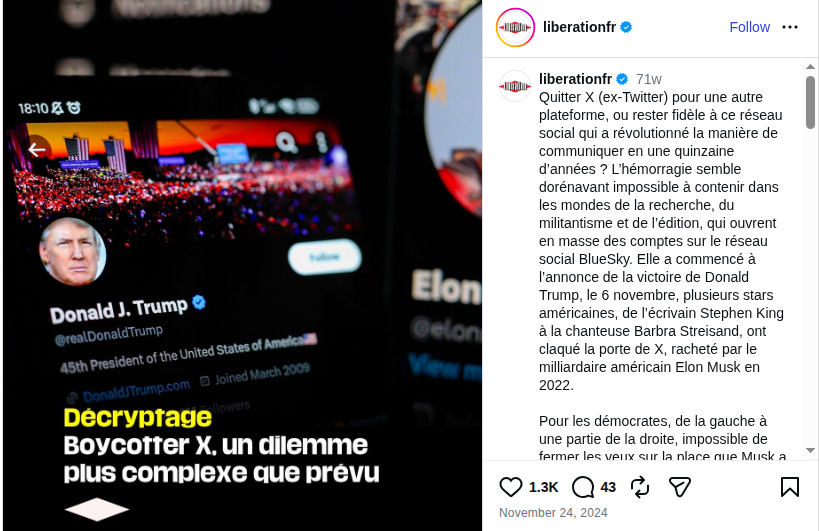
\includegraphics[width=.4\textwidth]{Images/libe_polémique_x.png}
    \end{figure}
\end{frame}

\begin{frame}{Une alternative possible: Patreon?}
    \begin{itemize}
        \item Création en 2013
        \item Plateforme de financement participatif (micro-contributions mensuelles)
    \end{itemize}
    \centering
    \begin{figure}
        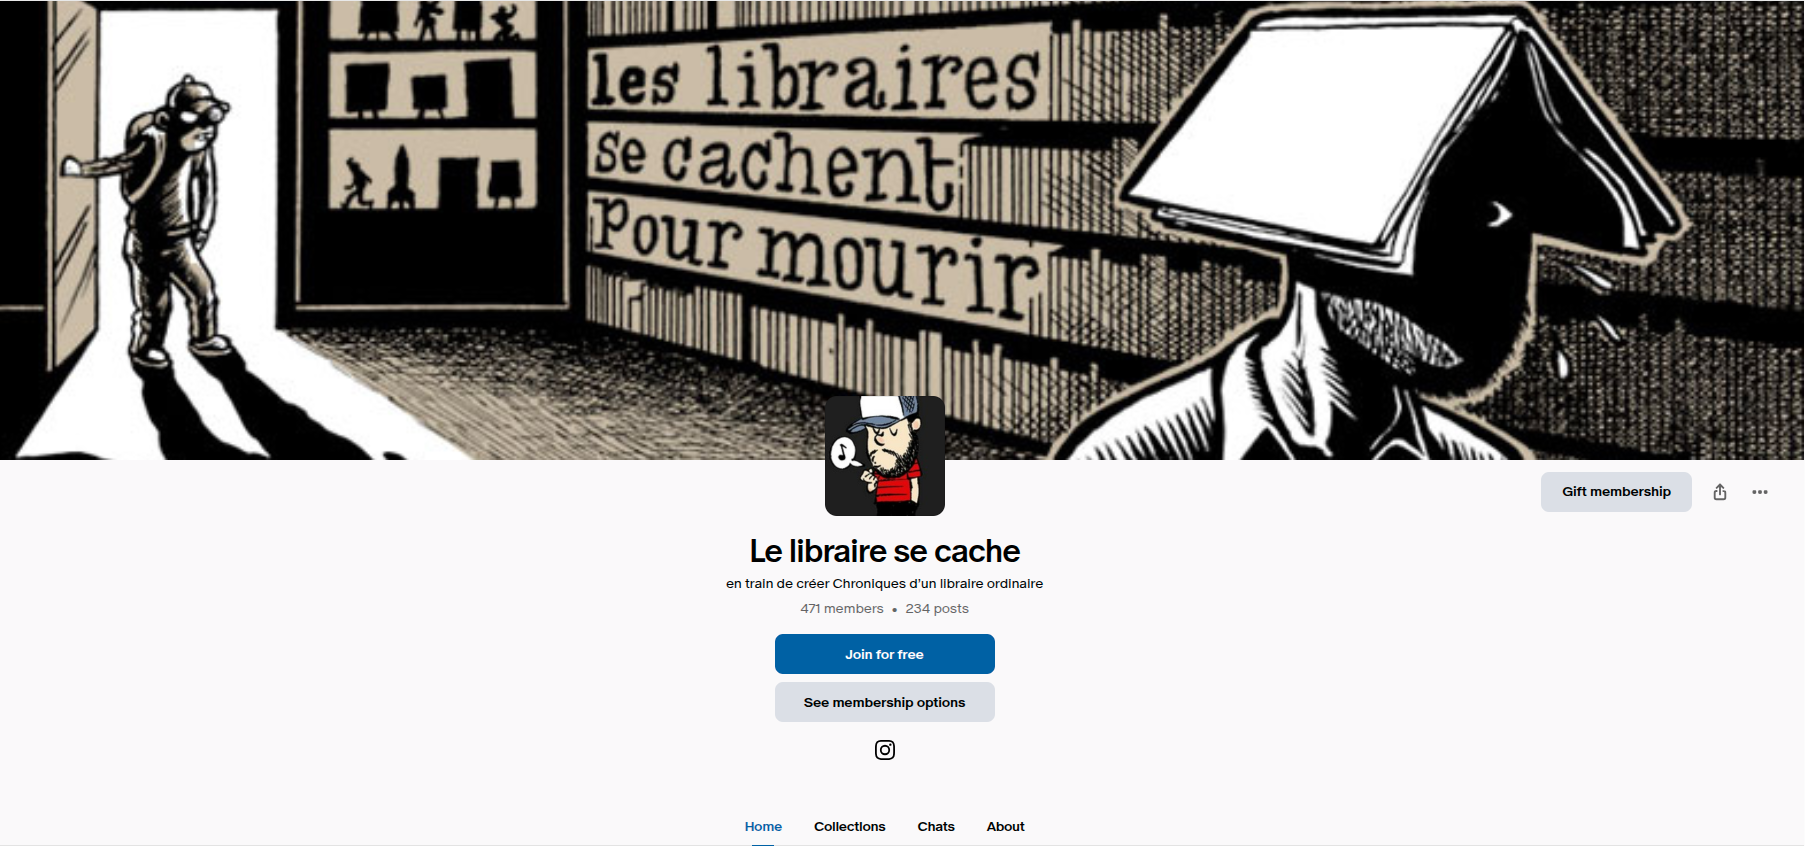
\includegraphics[width=.4\textwidth]{Images/patreon_libraire_se_cache.png}
        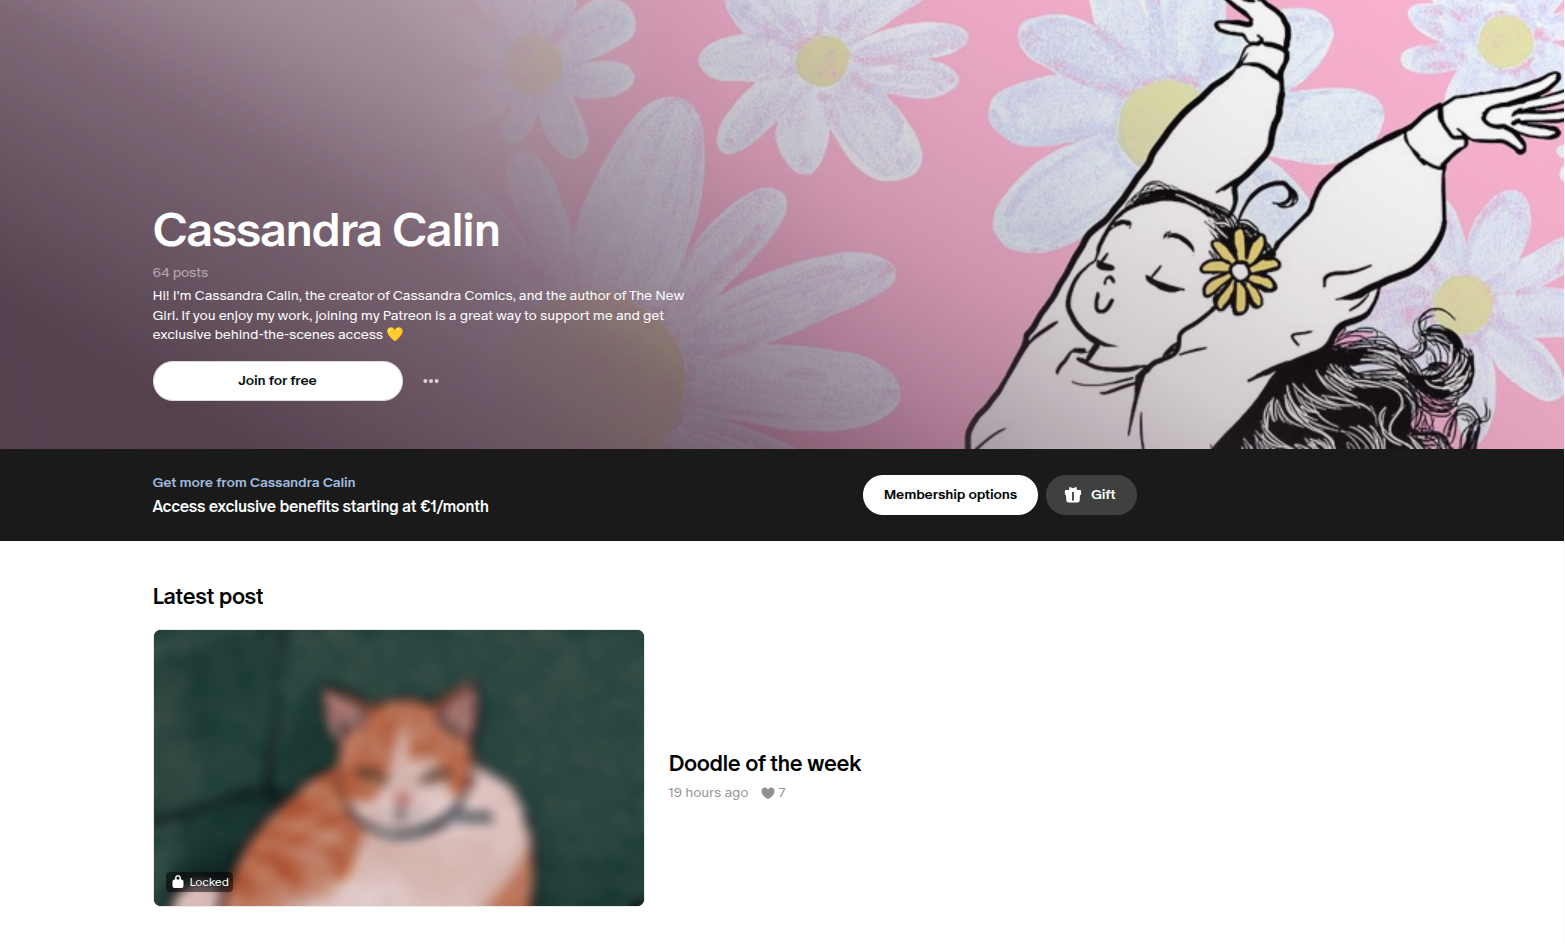
\includegraphics[width=.4\textwidth]{Images/patreon_cassandra_callin.png}
    \end{figure}
\end{frame}

